\subsection{Author-collected hypocotyl growth under a light--dark cycle}
\label{subsec:hypocotylresults}

On our author-collected hypocotyl dataset, \model{} again achieved the lowest mean test error among the compared baseline families. The experiment adds a distinct setting to the temperature-conditioned benchmarks: growth at constant 23~$^{\circ}$C under a known light--dark cycle, observed through unequal numbers of replicate plants at only seven times. The 943 measurements span five genotypes and are evaluated as 35 split-specific replicate means per partition. This tests prediction of genotype-level mean growth from sparse replicate snapshots.

Validation selected learning rate 0.01, $\lambda_{\mathrm{ODE}}=500$, $\lambda_K=0.1$, and weight decay $10^{-4}$ for the 1,103-parameter light-input \model{}. The model retains the ordinary logistic reference described in Section~\ref{subsec:lightmodel}; illumination drives the latent vector field, while the reference rate and capacity remain time-independent within each genotype.

Table~\ref{tab:hypocotyl_replicate} reports train, validation, and test RMSE / relative RMSE. \model{} achieved $0.3460\pm0.0077$~mm / $6.85\pm0.15\%$, compared with $0.3607\pm0.0136$~mm / $7.14\pm0.27\%$ for Logistic-PINN, the strongest baseline by mean test RMSE, and $0.3679\pm0.0070$~mm / $7.28\pm0.14\%$ for the no-physics latent ODE. These correspond to RMSE reductions of 4.07\% and 5.95\%, respectively. PhytoODE also attained the lowest mean validation RMSE among the six selected models, extending its benchmark-leading performance to measurements collected by the authors.

\begin{table}[t]
\centering
\small
\caption{Author-collected 12L12D hypocotyl dataset: replicate-group holdout. Each cell reports RMSE (mm) / relative RMSE (\%), as mean $\pm$ sample SD over three seeds; logistic ODE is fitted once. Metrics use the 35 split-specific replicate means in each partition. Bold denotes the smallest unrounded mean among these six selected models. PhytoODE uses the known binary light schedule and the configuration selected by validation; the five genotype-and-time baselines retain their preceding fits. Input and search procedures are described in Section~\ref{subsec:lightmodel}.}
\label{tab:hypocotyl_replicate}
\resizebox{\linewidth}{!}{%
\begin{tabular}{lccc}
\toprule
Model & Train & Validation & Test \\
\midrule
Logistic ODE & $0.370\,/\,7.29$ & $0.408\,/\,8.07$ & $0.485\,/\,9.61$ \\
Random forest & $0.364\pm0.013\,/\,7.17\pm0.26$ & $0.472\pm0.027\,/\,9.33\pm0.53$ & $0.452\pm0.014\,/\,8.95\pm0.28$ \\
LSTM-NN & $\mathbf{0.137\pm0.029\,/\,2.71\pm0.58}$ & $0.288\pm0.014\,/\,5.68\pm0.28$ & $0.361\pm0.007\,/\,7.15\pm0.14$ \\
Logistic-PINN & $0.219\pm0.013\,/\,4.32\pm0.26$ & $0.304\pm0.002\,/\,6.00\pm0.04$ & $0.361\pm0.014\,/\,7.14\pm0.27$ \\
Latent ODE (no physics) & $0.190\pm0.007\,/\,3.75\pm0.15$ & $0.297\pm0.003\,/\,5.86\pm0.06$ & $0.368\pm0.007\,/\,7.28\pm0.14$ \\
\model{} & $0.190\pm0.008\,/\,3.75\pm0.15$ & $\mathbf{0.278\pm0.001\,/\,5.48\pm0.02}$ & $\mathbf{0.346\pm0.008\,/\,6.85\pm0.15}$ \\
\bottomrule
\end{tabular}}
\end{table}


\begin{figure}[!htbp]
\centering
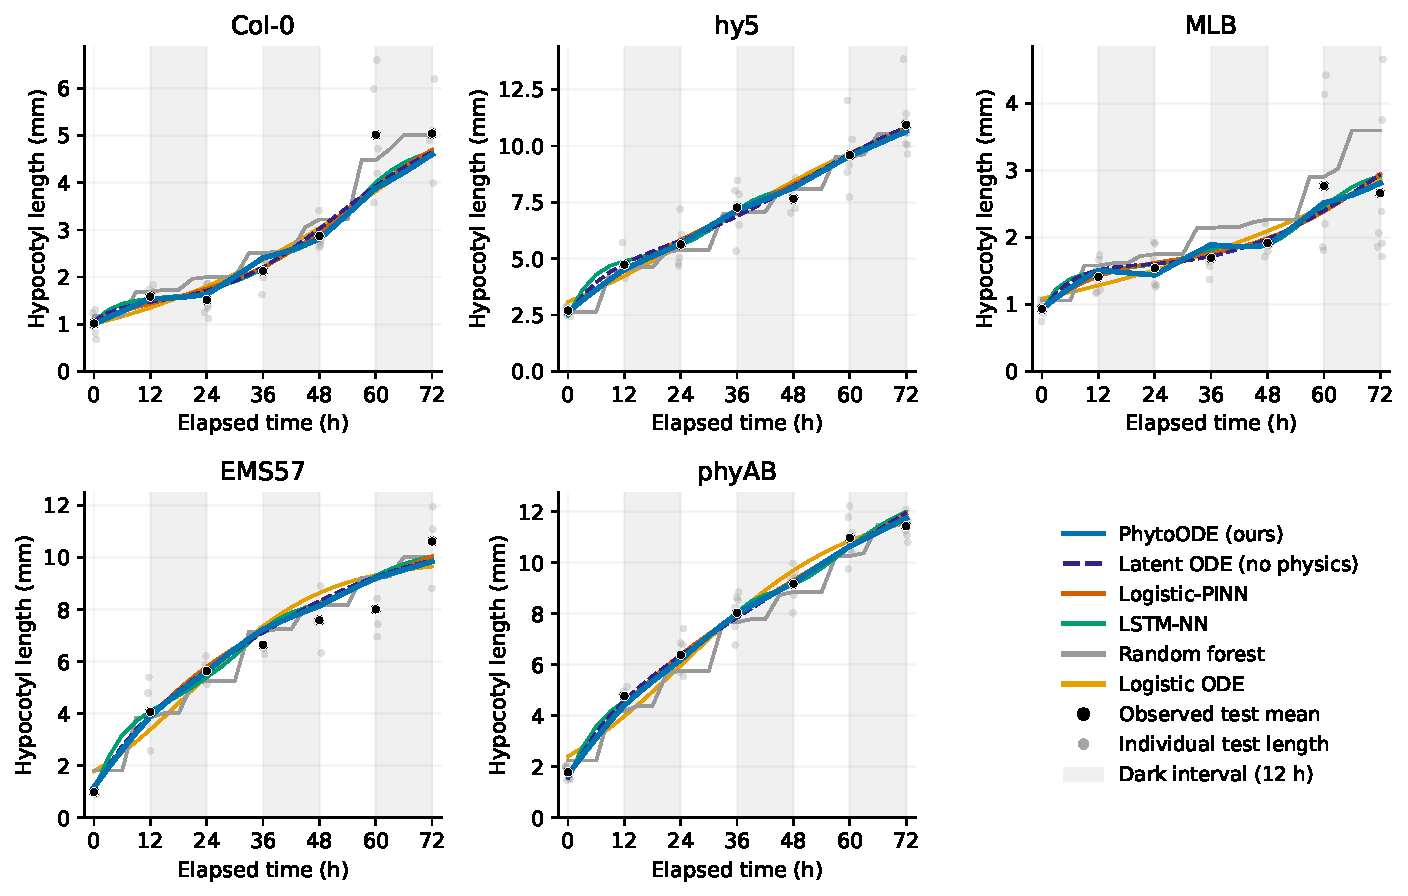
\includegraphics[width=\linewidth]{figures/hypocotyl_light_input.pdf}
\caption{Predicted hypocotyl growth for all five genotypes in the author-collected 12L12D experiment at 23~$^{\circ}$C. Blue curves show the validation-selected PhytoODE with binary illumination input and ordinary logistic regularization; the other methods receive genotype and elapsed time. Curves average predictions across three seeds, except the single-fit logistic ODE. Black points are test replicate means, and faint gray points show contributing individual measurements with small horizontal offsets for visibility. Shaded intervals denote darkness. Each split contains distinct replicate groups at all seven observed times. Model curves between these times do not represent additional measurements.}
\label{fig:hypocotyllight}
\end{figure}

Figure~\ref{fig:hypocotyllight} shows the five genotype-specific length curves. The shared model represents their different elongation magnitudes with a common light-phase input. Thus, the same latent ODE formulation accommodates illumination as well as temperature, while retaining a single logistic reference for each genotype. Sparse observations and unequal replicate counts enter through the split-specific targets and observation mask; blank spreadsheet cells are never replaced by artificial lengths.

A prespecified feature comparison retained the preceding PhytoODE hyperparameters and added only the light channel. Its test score was $0.3293\pm0.0057$~mm / $6.52\pm0.11\%$, compared with $0.3646\pm0.0079$~mm / $7.22\pm0.16\%$ without light input. The fixed-settings light-input variant had lower test error than the subsequently tuned variant, but its mean validation RMSE was higher ($0.2886$ versus $0.2777$~mm). The main table therefore retains the configuration chosen by validation. These additional comparisons support the usefulness of the explicit phase feature under the recorded procedures; the retained no-light baselines and unequal tuning budgets do not isolate a physics-loss effect.

As a secondary evaluation against individual test lengths, pooled RMSE was $0.7328$~mm for \model{} and $0.7394$~mm for the no-physics latent ODE. These values include within-group biological variation and use a different aggregation rule from the primary mean-trajectory metric. The primary result concerns held-out replicate means in one genotype panel and one prescribed photoperiod; independent batches and additional photoperiods would test broader transfer.

Beyond predictive accuracy, this experiment contributes an original dataset for reproducible comparison. The planned public release links each retained measurement to its workbook cell and includes fixed partitions, target-construction code, model configurations, validation histories, and predictions. It will allow subsequent methods to use the same sparse sampling pattern and replicate-level evaluation protocol.

Halving the integration step from 3 to 1.5~h, with the encoder inputs held fixed, changed the selected PhytoODE predictions by at most $2.5\times10^{-6}$~mm across the three seeds.

\FloatBarrier
